\chapter{Falsifiable benchmark와 experiment roadmap}
\label{STC-S15}

이 분야에 필요한 다음 산출물은 더 큰 metaphor가 아니라 matched lifecycle experiment다. 같은 wake
events와 future queries를 주고, exact external retention, external compaction, latent/KV compilation,
user-local adapter, deliberate forgetting, past-only hybrid routing 중 무엇이 가장 나은지를 측정해야 한다.
Null result와 boundary를 계획에 포함해야 negative paper도 가치가 있다.

\begin{figure}[htbp]
  \centering
  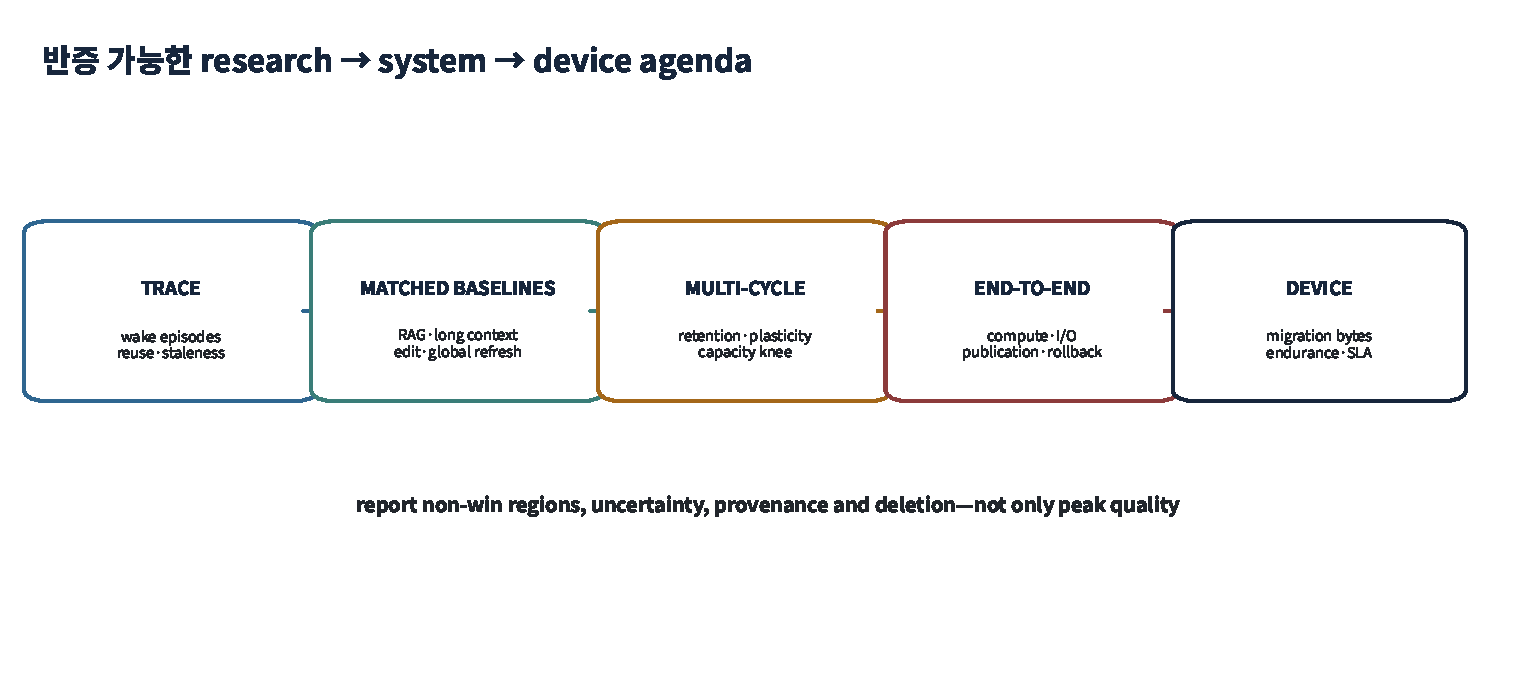
\includegraphics[width=0.98\textwidth]{figures/stc-f015.pdf}
  \caption{Falsifiable research agenda. Evidence stream, candidate construction, lifecycle validation,
  repeated-cycle evaluation, scaling fit을 하나의 provenance chain으로 연결한다.}
  \stcfigure{STC-F015}
  \figsource{Original synthesis; SRC-STC-0036, SRC-STC-0050, SRC-STC-0056}{Matched methods, cycle probes, systems/governance metrics, held-out scaling test가 순차적으로 이어지는 roadmap.}
  \label{fig:benchmark-agenda}
\end{figure}

\section{독립 단위와 cycle}

최상위 independent unit은 user/stream이다. Cycle과 probe를 독립 sample처럼 세어 significance를
부풀리지 않는다. 한 cycle은 다음 순서를 가진다.

\begin{align*}
\text{wake capture}&\rightarrow\text{pre-sleep probe}\rightarrow
\text{immutable snapshot}\rightarrow\text{candidate}\\
&\rightarrow\text{validate/publish}\rightarrow\text{post-sleep probe}
\rightarrow\text{delayed next-wake probe}.
\end{align*}

Default horizon은 128 cycles, sensitivity는 $C\in\{8,32,128,512\}$, retrieval lag는 가능한 경우
$\{1,8,32,128\}$ cycles로 둔다. 단일 sleep 후 정확도는 lifelong behavior를 지지하지 못한다.

\section{Observable과 oracle을 물리적으로 분리한다}

Method가 보는 observable stream에는 event payload, 현재 confidence, privacy scope, 알려진
supersession/delete, past reuse, resource/queue state만 있다. True future reuse, future contradiction,
future deletion, poison truth, ground-truth dependency, clairvoyant destination은 oracle ledger에 따로 둔다.
파일, schema, API permission과 process boundary로 누출을 막는다.

Train은 learned router/compiler를 fit하고, CALIBRATION은 threshold, cadence, baseline hyperparameter를
한 번 선택하며, TEST는 G2 freeze 뒤 한 번만 실행한다. TEST family identity나 future reuse로 configuration을
바꾸는 mutation test가 통과해야 한다. Dream-generated probe도 evaluation query가 아니라 derived training
artifact이므로 generator/prompt/input/output/filter digest를 남긴다.

\section{Event와 query family}

\begin{table}[htbp]
\centering
\caption{독립적으로 변화시킬 event factor와 주요 failure}
\label{tab:event-families}
\begin{tabularx}{\textwidth}{L{0.23\textwidth} L{0.34\textwidth} Y}
\toprule
Family & Controlled variables & 잡아야 할 failure \\
\midrule
stable exact fact & entropy, surface length, reuse, lag & semantic compression이 exact detail을 지움 \\
volatile fact/preference & validity interval, correction hazard & stale overwrite, historical loss \\
procedure/skill & reusable/one-off, environment version & vague summary, non-executable memory \\
relation/graph & alias, temporal edge, hop count & entity collision, invalid edge \\
failure feedback & wrong action, correction, avoidance & success-only bias \\
privacy/delete & consent expiry, dependency fan-out & tombstone-only delete \\
poison/adversarial & injection, conflicting frequency, delayed label & poison amplification \\
one-off distractor & salience, payload size, zero reuse & unnecessary consolidation \\
\bottomrule
\end{tabularx}
\end{table}

Reuse, volatility, poison, deletion, payload size와 memory pressure는 서로 독립적으로 변화시킨다. Query는
exact, semantic, temporal, relational, procedural, negative/failure, calibration, deletion family로 나눈다.
Acquisition query, exact repeat, held-out paraphrase, held-out composition, correction probe, unrelated control을
동일 지표로 합치지 않는다. ``기억한 문장을 그대로 다시 답했다''와 ``새 상황에 procedure를 적용했다''는
다른 능력이다.

\section{Confirmatory methods와 resource envelope}

Primary deployable family는 raw external, compressed external, latent/KV compiler, user-parametric LoRA,
static mixture, past-only hybrid router 여섯 개다. Clairvoyant oracle은 heterogeneity의 upper bound일 뿐
deployable method가 아니다. Long-context no-memory lower bound와 unbounded full-history upper bound는
diagnostic으로 남긴다.

모든 method는 다음 upper bound를 공유한다.

\begin{itemize}
  \item live token, active byte, durable byte, total incremental peak-state byte,
  \item physical HBM/fleet peak, sleep FLOPs, peak accelerator,
  \item 동일한 information cutoff, privacy와 delete contract.
\end{itemize}

Search/tuning, router, judge, embedding, synthetic data, optimizer, answer-reachable KV/recurrent state, index
rebuild, raw archive, lineage, rollback reserve와 transient workspace를 모두 charge한다. 사용하지 않은 budget은
낭비하도록 강제하지 않고 그대로 보고한다.

Reuse $R\in\{0,1,4,16\}$와 active-capacity ratio
$\phi\in\{1,1/4,1/16\}$을 교차한다. Schedule/operator factorial은 inline versus deferred와 identity
versus semantic consolidation을 destination external로 고정해, execution timing의 효과와 추가 정보를 더
본 효과를 분리한다.

\section{Metric stack}

\begin{longtable}{L{0.17\textwidth} L{0.74\textwidth}}
\caption{한 결과표에 함께 있어야 할 metric stack}\label{tab:benchmark-metrics}\\
\toprule
Layer & Required metrics \\
\midrule
\endfirsthead
\toprule
Layer & Required metrics \\
\midrule
\endhead
learning & lifetime utility AUC, current utility, acquisition, retention/forgetting, forward transfer, memory half-life \\
semantic & exact/semantic/temporal/relational/procedural, composition, relevance, calibration, false memory \\
memory path & writer/retriever/reader error, route/merge compatibility, coverage, faithfulness, detail loss, stale conflict \\
robustness & poison amplification, cross-user/task interference, rare-tail survival, recursive-depth distortion \\
governance & access deny, physical removal, lineage invalidation, key expiry, behavioral residual, rollback success/time \\
serving & TTFT/ITL/task P50/P95/P99, throughput, cache/adapter hit, load/swap, fallback \\
sleep service & throughput, queue age, deadline miss, retry, validation/publish/rollback cost \\
resources & pre/post/wake/sleep/validation FLOPs, retained/peak bytes, bytes moved by link, write amplification, energy \\
compatibility & base/tokenizer/embedding version, artifact route, rebase and rebuild cost \\
\bottomrule
\end{longtable}

Primary quality endpoint은 cycle과 pre/post/delayed probe block에 동일 가중치를 주는 lifetime utility AUC다.
Energy-per-correct는 frozen accuracy floor 위에서만 계산한다. Delete score는 access denial과 physical removal,
derived invalidation, behavioral residual을 한 binary로 합치지 않는다.

\section{통계·재현성과 claim-down rule}

모든 method는 같은 stream, event order, query order, resource tuple을 받는다. User/stream을 paired resampling
unit로 사용하고 workload-family$\times$seed-family block을 유지한다. Hardware placement와 method order는
randomize 또는 block한다. Outcome을 본 뒤 stopping point, comparator, hypothesis family를 바꾸지 않는다.

Run artifact는 source/version $\rightarrow$ question/hypothesis $\rightarrow$ config/data/code/environment
$\rightarrow$ raw checksum $\rightarrow$ result $\rightarrow$ claim $\rightarrow$ figure/table
$\rightarrow$ manuscript sentence를 연결한다. Timeout, OOM, deadline miss, cap violation은 missing data가
아니라 consumed work를 charge한 RESOURCE\_FAILURE로 처리한다.

다음 경우 claim을 낮춘다: effect가 materiality margin보다 작음, equivalence interval이 margin을 걸침,
simulation으로 absolute hardware latency를 말함, archive를 남기고 total compression이라 함, behavioral
forgetting을 physical deletion이라 함, post-hoc arm을 추가함. Minimum publishable result는 hybrid가
실패해도 deterministic leakage-tested stream, matched methods, complete resource ledger, retention/acquisition
분리와 잘 추정된 crossover·knee·null 중 하나를 남기는 것이다.

\begin{keypoint}[실험의 최종 질문]
``Sleep이 정확도를 높였는가?''가 아니라 ``동일한 evidence와 lifetime budget에서, 어떤 admission,
operator, destination, cadence가 later-wake utility와 governance의 Pareto frontier를 움직였는가?''를 묻는다.
\end{keypoint}
